\documentclass{llncs}
\usepackage{amsmath,amssymb,calc,ifthen}
\usepackage{float}
%\usepackage{cancel}
\usepackage[table,usenames,dvipsnames]{xcolor} % for coloured cells in tables
\usepackage{tikz}
% Allows us to click on links and references!
\usepackage{hyperref}
\usepackage{url}
\hypersetup{
colorlinks,
citecolor=black,
filecolor=black,
linkcolor=black,
urlcolor=black
}
% Nice package for plotting graphs
% See excellent guide:
% http://www.tug.org/TUGboat/tb31-1/tb97wright-pgfplots.pdf
\usetikzlibrary{plotmarks,shapes}
\usepackage{amsmath,graphicx}
\usepackage{epstopdf}
%\usepackage{caption}
\usepackage{subcaption}
\usepackage{graphicx}
% highlight - useful for TODOs and similar
\usepackage{color}
\newcommand{\hilight}[1]{\colorbox{yellow}{#1}}
\newcommand\ci{\perp\!\!\!\perp} % perpendicular sign
\newcommand*\rfrac[2]{{}^{#1}\!/_{#2}} % diagonal fraction
\newcommand\SLASH{\char`\\}
\usepackage{listings}
% margin size
\usepackage{pdfpages}
\usepackage{enumitem} % for nested enumerate numbers 1 1.1 1.1.1
% \usepackage{breqn}
% \usepackage[linesnumbered]{algorithm2e}
% \usepackage{algorithmicx,algpseudocode}
% \usepackage{wrapfig} % for allowing text wrapped around the algorithm
% \newcommand\mycommfont[1]{\footnotesize\ttfamily\textcolor{blue}{#1}}
% \SetCommentSty{mycommfont}

% \usepackage{titlesec}
% \titlespacing*{\section}
% {0pt}{5.5ex plus 1ex minus .2ex}{4.3ex plus .2ex}

\usepackage[linesnumbered,noend]{algorithm2e}
\newcommand\mycommfont[1]{\footnotesize\ttfamily\textcolor{blue}{#1}}
\SetCommentSty{mycommfont}

\setlength{\textfloatsep}{15pt}
%\setlength{\floatsep}{1pt}
%\setlength{\topmargin}{1pt}

\renewcommand\floatpagefraction{.95}
\renewcommand\topfraction{.95}
\renewcommand\bottomfraction{.95}
\renewcommand\textfraction{.05}   
\setcounter{totalnumber}{50}
\setcounter{topnumber}{50}
\setcounter{bottomnumber}{50}

\DeclareMathOperator*{\argmin}{arg\,min}
\DeclareMathOperator*{\argmax}{arg\,max}

\begin{document}

\definecolor{blue3}{HTML}{86B7FC} % med blue
\definecolor{blue1}{HTML}{B5F1FF} % light blue
\definecolor{blue2}{HTML}{E0F9FF} % very light blue

\title{Disease Knowledge Transfer across Neurodegenerative Diseases}
%
\titlerunning{Disease Knowledge Transfer across Neurodegenerative Diseases}  % abbreviated title (for running head)
%                                     also used for the TOC unless
%                                     \toctitle is used
%

% * <mrazvan22@gmail.com> 2018-03-02T16:41:47.321Z:
% 
% Author list: Me, Marco (writing+model code), Stefano, Alex Young (writing+tadpole), Pere (helped with validation),Neil (tadpole),  Arman, Keir (DTI data), Seb, Danny
% 
% ^ <mrazvan22@gmail.com> 2018-03-02T16:55:06.003Z.

\author{R\u{a}zvan V. Marinescu\inst{1} \and Marco Lorenzi\inst{1,4} \and Stefano Blumberg\inst{1} \and 
 Alexandra L. Young\inst{1} \and Pere P. Morell\inst{1} \and Neil P. Oxtoby\inst{1} \and Arman Eshaghi\inst{1,2} \and Keir X. Yong\inst{3} \and Sebastian J. Crutch\inst{3} \and Daniel C. Alexander\inst{1}, for 
the  Alzheimer’s  Disease  Neuroimaging Initiative
% \thanks{Data used in preparation of this article were obtained from the Alzheimer's Disease Neuroimaging Initiative (ADNI) database (adni.loni.usc.edu). As such, the investigators within the ADNI contributed to the design and implementation of ADNI and/or provided data but did not participate in analysis or writing of this report. A complete listing of ADNI investigators can be found at: http://adni.loni.usc.edu/wp-content/uploads/how\_to\_apply/ADNI\_Acknowledgement\_List.pdf}
}

\authorrunning{R\u{a}zvan V. Marinescu et al.} % abbreviated author list (for running head)

\institute{Centre for Medical Image Computing, University College London, UK
\and 
Queen Square MS Centre, UCL Institute of Neurology, UK
\and 
Dementia Research Centre, University College London, UK
\and
University of C\^{o}te d'Azur, Inria Sophia Antipolis, France
% Laboratoire d'Analyse Num\'{e}rique, B\^{a}timent 425,\\
% F-91405 Orsay Cedex, France}
}


\maketitle              % typeset the title of the contribution


%\newcommand{\expFld}{../resfiles/tad-drcTiny_JMD}
\newcommand{\expFld}{.}

\begin{abstract}
We introduce Disease Knowledge Transfer (DKT), a novel technique for transferring biomarker information between related neurodegenerative diseases. DKT infers robust multimodal biomarker trajectories in rare neurodegenerative diseases even when only limited, unimodal data is available, by transferring information from larger multimodal datasets from common neurodegenerative diseases. DKT is a joint-disease generative model of biomarker progressions, which exploits biomarker relationships that are shared across diseases. As opposed to current deep learning approaches, DKT is interpretable, which allows us to understand underlying disease mechanisms, and can also predict the future evolution of subjects instead of solving simpler control vs diseased classification tasks. Here we demonstrate DKT on Alzheimer's disease (AD) variants and its ability to predict trajectories for multimodal biomarkers in Posterior Cortical Atrophy (PCA), in lack of such data from PCA subjects. For this we train DKT on a combined dataset containing subjects with two distinct diseases and sizes of data available: 1) a larger, multimodal typical AD (tAD) dataset from the TADPOLE Challenge, and 2) a smaller unimodal Posterior Cortical Atrophy (PCA) dataset from the Dementia Research Centre (DRC) UK, for which only a limited number of Magnetic Resonance Imaging (MRI) scans are available. We first show that the estimated multimodal trajectories in PCA are plausible as they agree with previous literature. We further validate DKT in two situations: (1) on synthetic data, showing that it can accurately estimate the ground truth parameters and (2) on 20 DTI scans from controls and PCA patients, showing that it has favourable predictive performance compared to standard approaches. While we demonstrated DKT on Alzheimer's variants, we note DKT is generalisable to other forms of related neurodegenerative diseases.

\keywords{Disease Progression Model, Transfer Learning, Manifold Learning, Alzheimer's Disease, Posterior Cortical Atrophy}
\end{abstract}

\section{Introduction}


The estimation of accurate biomarker signatures in Alzheimer's disease (AD) and related neurodegenerative diseases is crucial for understanding underlying disease mechanisms, predicting subjects' progressions, and enrichment in clinical trials. Recently, data-driven disease progression models were proposed to reconstruct long term biomarker signatures from collections of short term individual measurements \cite{lorenzi2017disease,oxtoby2018,jedynak2012computational}. When applied to large datasets of typical AD, disease progression models have shown important benefits in understanding the earliest events in the AD cascade \cite{oxtoby2018}, quantifying biomarkers' heterogeneity \cite{young2018uncovering} and they showed improved predictions over standard approaches \cite{oxtoby2018}. However, by necessity these models require large datasets -- in addition they should be both multimodal and longitudinal. Such data is not always available in rare neurodegenerative diseases. In particular, most datasets for rare neurodegenerative diseases come from local clinical centres, are unimodal (e.g. MRI only) and limited both cross-sectionally and longitudinally -- this makes the application of disease progression models extremely difficult.  Moreover, such a model estimated from common diseases such as typical AD may not generalise to specific variants. For example, in Posterior Cortical Atrophy (PCA) -- a neurodegenerative syndrome causing visual disruption -- posterior regions such as the occipital lobe are affected early, instead of the hippocampus and temporal regions in typical AD. 

The problem of limited data in medical imaging has so far been addressed through transfer learning methods. These were successfully used to improve the accuracy of AD diagnosis \cite{hon2017towards} or prediction of MCI conversion \cite{cheng2015domain}, but have two key limitations. First, they use deep learning or other machine learning methods, which are not interpretable and don't allow us to understand underlying disease mechanisms that are either specific to rare diseases, or shared across related diseases. Secondly, these models cannot be used to forecast the future evolution of subjects at risk of disease, which is important for selecting the right subjects in clinical trials. 

We propose Disease Knowledge Transfer (DKT), a generative joint model that estimates continuous multimodal biomarker progressions for multiple diseases simultaneously -- including rare neurodegenerative diseases -- and which inherently performs transfer learning between the modelled phenotypes. This is achieved by exploiting biomarker relationships that are shared across diseases, whilst accounting for differences in the spatial distribution of brain pathology. DKT is interpretable, which allows us to understand underlying disease mechanisms, and can also predict the future evolution of subjects at risk of diseases. We apply DKT on Alzheimer's variants and demonstrate its ability to predict non-MRI trajectories for patients with Posterior Cortical Atrophy, in lack of such data. This is done by fitting DKT to two datasets simultaneously: (1) the TADPOLE Challenge \cite{marinescu2018tadpole} dataset containing subjects from the Alzheimer's Disease Neuroimaging Initiative (ADNI) with MRI, FDG-PET, DTI, AV45 and AV1451 scans and (2) MRI scans from patients with Posterior Cortical Atrophy from the Dementia Research Centre (DRC), UK. We first show that the estimated trajectories for PCA and tAD subjects are plausible as they agree with previous literature findings. We finally validate DKT on simulated data from two synthetic diseases with known ground truth, and a set of 20 DTI scans from controls and PCA patients.

\begin{figure}[h]
 \centering
 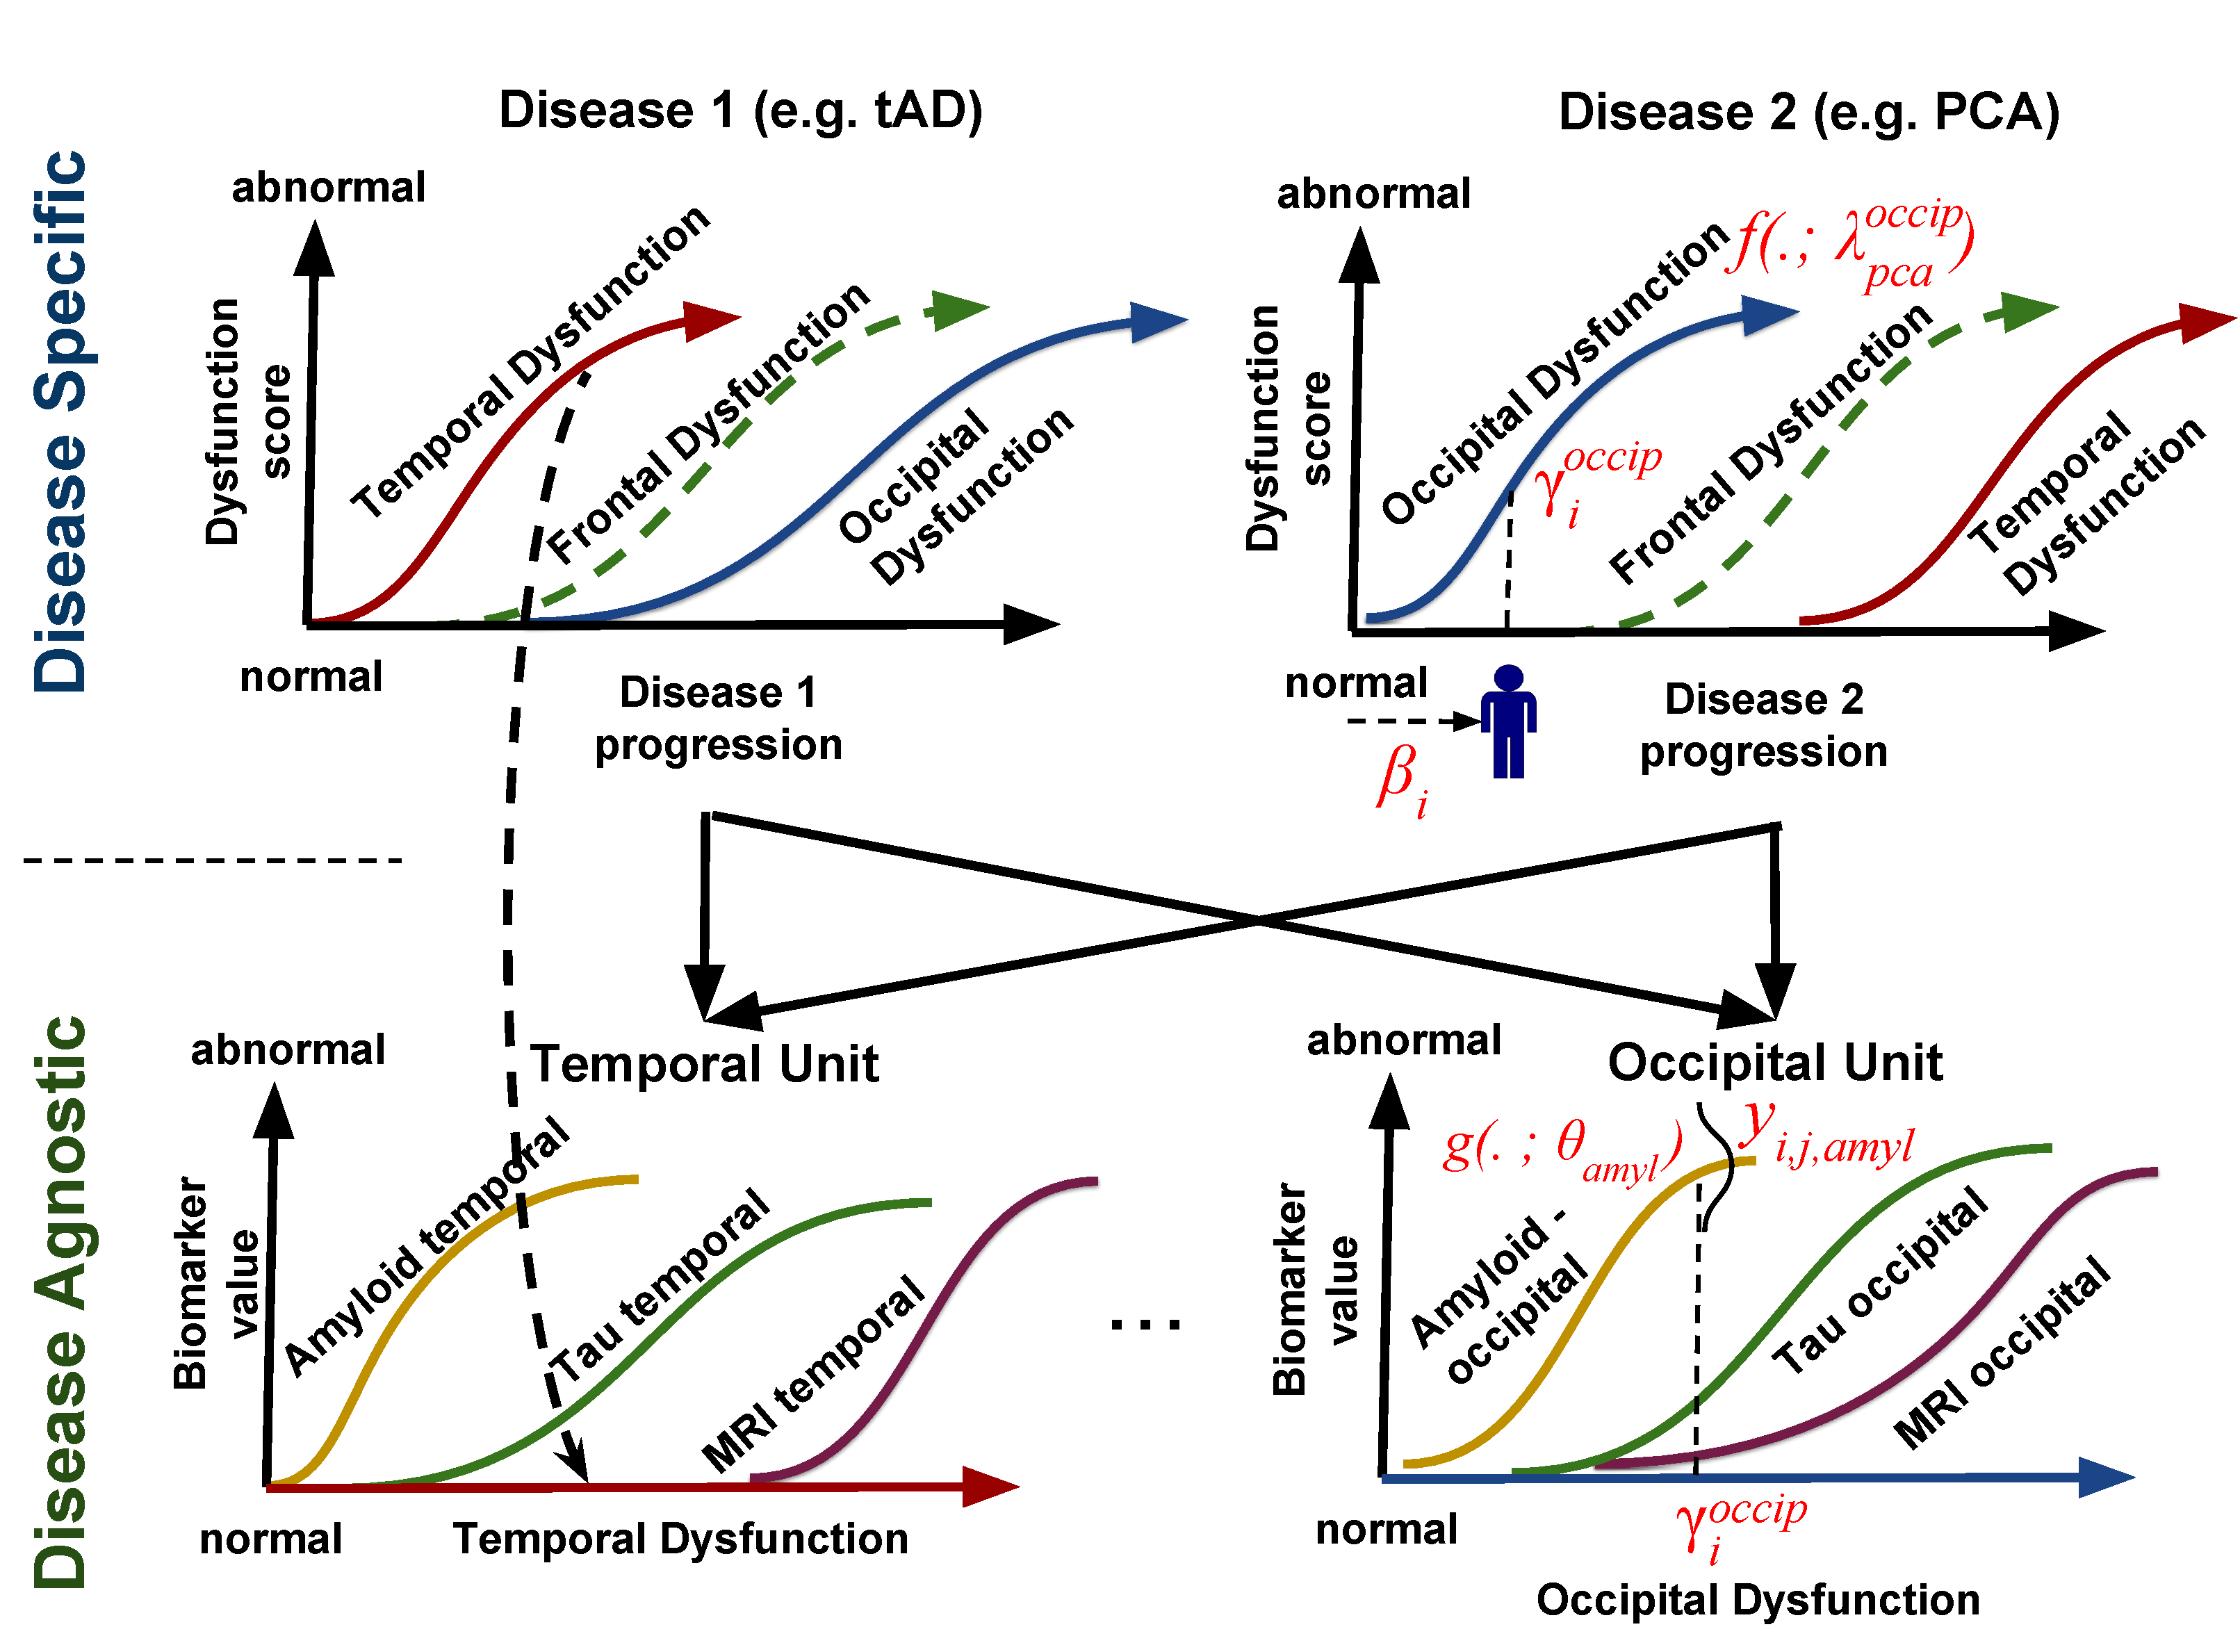
\includegraphics[width=0.8\textwidth,trim=0 0 0 0,clip]{disease_knowledge_transfer_symbols.pdf}
 \caption{Diagram of the proposed DKT framework. We assume that each disease can be modelled as the evolution of abstract dysfunction scores (Y-axis, top row), each one related to different brain regions. Each region-specific dysfunction score then further models (X-axis, bottom row) the progression of several modality-specific biomarkers within that same region. For instance, the temporal dysfunction, modelled as a biomarker in the disease specific model (top row), is the X-axis in the disease agnostic model (temporal unit, bottom row), which aggregates together abnormality from amyloid, tau and MR imaging within the temporal lobe. The biomarker relationships within the bottom units are assumed to be disease agnostic and shared across all diseases modelled. Knowledge transfer between the two diseases can then be achieved via the disease-agnostic units. Mathematical notation from section \ref{sec:method} is shown in red to ease understanding.}
 \label{fig:diagram}
\end{figure}

\section{Method}
\label{sec:method}

\subsection{Method Overview}

\newcommand{\lp}{\lambda_{d_i}^{\psi(k)}}
\newcommand{\lpuu}{\lambda_{d_i}^{\psi(k),(u)}}
\newcommand{\lpum}{\lambda_{d_i}^{\psi(k),(u-1)}}

Fig. \ref{fig:diagram} shows the overall diagram of the DKT framework. We assume that the progression of each disease (X-axis, top row) can be modelled as a unique evolution of dysfunction trajectories (top row) representing multimodal pathology within a specific brain region. Each dysfunction trajectory is modelled as the progression of several biomarkers within that same region, but acquired using different types of modalities (e.g. MRI, PET or DTI, see Fig. \ref{fig:diagram} bottom row). Each group of biomarkers in the bottom row will be called a \emph{disease-agnostic unit} or simply \emph{agnostic unit}, because the biomarker dynamics are assumed to be shared across all diseases modelled.

The assumption that the dynamics of some biomarkers are disease-agnostic (i.e. shared across diseases), is key to DKT. There are several reasons why we can make this assumption. First of all, pathology in many related neurodegenerative diseases ( e.g. Alzheimer's variants) are hypothesised to share the same underlying mechanisms (e.g. amyloid and tau accumulation), and within one region, such accumulation leads to the same pathology dynamics across all the related disease variants: hypometabolism (FDG PET), neuronal damage (T1/DTI MRI) and region-specific cognitive decline \cite{jack2010hypothetical} -- the difference between these variants is that distinct brain regions are affected at different times and with different pathology rates and extent, likely caused by selective vulnerability of networks within these regions \cite{seeley2009neurodegenerative}. Secondly, even if the diseases share different upstream mechanisms (e.g. amyloid vs tau accumulation), downstream biomarkers measuring hypometabolism, white matter degradation and structural markers follow the same pathological cascade and will have similar dynamics across diseases.

We choose to model the correlations within each agnostic unit using the disease progression model (DPM) by \cite{jedynak2012computational}, but any other DPM can also be used. The DPM allows us to reconstruct unit-specific dysfunction progression manifolds (bottom row, X axis), which can be used for staging subjects. Finally, we use the same model to express the progression within each disease (Figure 1, top) in terms of the dysfunction scores estimated within each agnostic unit. More precisely, the X-axis dysfunction scores from the agnostic units become Y-axis measurements in the disease specific models.

% \subsection{Disease-Specific Model}

In this section we model the biomarker dynamics that are specific to each disease, by mapping the subjects' disease stages to dysfunction scores. We model the progression of related diseases as the unique dynamics of abstract dysfunction scores, which aggregate together data from multiple biomarkers. We assume that each subject $i$ at each visit $j$ has an underlying disease stage $s_{ij} = \beta_i + m_{ij}$, where $m_{ij}$ represents the months since baseline visit for subject $i$ at visit $j$ and $\beta_i$ represents the time shift of subject $i$. We then assume that each subject $i$ has a dysfunction score $\gamma_i^l$ corresponding to multimodal pathology in brain region $l$, which is a function of its disease stage:

\begin{equation}
\label{eqDysfunctionScoreDef}
 \gamma_i^l = f(\beta_i + m_{ij}; \lambda_{d_i}^l)
\end{equation}
where $f$ is a smooth monotonic function mapping each disease stage to a dysfunction score, having parameters $\lambda_{d_i}^l$ corresponding to agnostic unit $l \in \Lambda$, where $\Lambda$ is the set of all agnostic units. Moreover, $d_i \in \mathbb{D}$ represents the index of the disease corresponding to subject $i$, where $\mathbb{D}$ is the set of all diseases modelled. For example, MCI and tAD subjects from ADNI as well as tAD subjects from the DRC cohort can all be assigned $d_i=1$, while PCA subjects can be assigned $d_i=2$.  We implement $f$ as a parametric sigmoidal curve similar to \cite{jedynak2012computational}, to enable a robust optimisation and because this accounts for floor and ceiling effects present in AD biomarkers. Variable $\epsilon_k$ denotes the variance of measurements for biomarker $k$. 

% \subsection{Disease-Agnostic Model}

We model the biomarker dynamics that are disease-agnostic, by constructing the mapping from the dysfunction scores $\gamma_i^l$ to the biomarker measurements. We assume a set of given biomarker measurements $Y = [y_{ijk} | (i,j,k) \in \Omega]$ for subject $i$ at visit $j$ in biomarker $k$, where $\Omega$ is defined as the set of available biomarker measurements, since subjects can have missing biomarkers at various visits. We further denote by $\theta_k$ the trajectory parameters for biomarker $k \in K$ within its agnostic unit $\psi(k)$, where $\psi$: \{1, ..., K\} $ \rightarrow \Lambda$ maps each biomarker $k$ to a unique agnostic unit $l \in \Lambda$. These definitions allow us to formulate the likelihood for a single measurement $y_{ijk}$ as follows:


\begin{equation}
 p(y_{ijk}|\theta_k, \lp, \beta_i, \epsilon_k) = N(y_{ijk}| g( \gamma_i^{\psi(k)} ; \theta_k), \epsilon_k)
\end{equation}
where $g(\ .\ ; \theta_k)$ represents the trajectory of biomarker $k$ within agnostic unit $\psi(k)$. Parameters $\lp$ are used to define $\gamma_i^{\psi(k)}$ based on Eq. \ref{eqDysfunctionScoreDef}, where agnostic unit $l$ is now referred to as $\psi(k)$, to clarify that this is the unit where biomarker $k$ has been allocated. 

% \subsection{Extending to Multiple Subjects and Biomarkers}

We extend the above model to multiple subjects, visits and biomarkers to get the full model likelihood:
\begin{equation}
 p(\boldsymbol{y}|\theta, \lambda, \beta , \epsilon) = \\ \prod_{(i,j,k) \in \Omega} p(y_{ijk}|\theta_k, \lp, \beta_i) 
\end{equation}
where $\boldsymbol{y} = [y_{ijk} | \forall (i,j,k) \in \Omega ]$ is the vector of all biomarker measurements, while $\boldsymbol{\theta} = [\theta_1, ..., \theta_K]$ represents the stacked parameters for the trajectories of biomarkers in agnostic units, $\boldsymbol{\lambda} = [\lambda_d^{l}|l \in \Lambda, d \in \mathbb{D}]$ are the parameters of the dysfunction trajectories within the disease models, $\boldsymbol{\beta} =[\beta_1, ..., \beta_N]$ are the subject-specific time shifts and $\boldsymbol{\epsilon} = [\epsilon_k | k \in K]$  estimates biomarker measurement noise. Here we assumed independence across different subjects, but the biomarker measurements and visits are linked through the latent time-shift $\beta_i$ for each subject. The parameters of the model that need to be estimated are $[\boldsymbol{\theta}, \boldsymbol{\lambda}, \boldsymbol{\beta}, \boldsymbol{\epsilon}]$.

We estimate the model parameters using a two-stage approach. In the first stage, we perform belief propagation within each agnostic unit and then within each disease model. In the second stage we jointly optimise across all agnostic units and disease models using loopy belief propagation.

%The sigmoidal model for $f$ is defined as:
%
%\begin{equation}
% f(s;\theta_k) = \frac{a_k}{1+exp(-b_k(s-c_k))} + d_k
%\end{equation}
%where $s$ is the disease progression score of a subject and $\theta_k = [a_k, b_k, c_k, d_k]$ are parameters controlling the shape of the trajectory for biomarker $k$: $d_k$ and $d_k + a_k$ represent the lower and upper limits of the sigmoidal function, $c_k$ represents the inflection point and $a_k b_k/4$ represents the slope at the inflection point. A similar model is used also for $g$.


% \subsection{Parameter Estimation}
% 
% \newcommand{\uu}{^{(u)}}
% \newcommand{\um}{^{(u-1)}}
% 
% We estimate the model parameters using a two-stage approach. In the first stage, we perform belief propagation within each agnostic unit and then within each disease model. In the second stage we jointly optimise across all agnostic units and disease models using loopy belief propagation. An overview of the algorithm is given in Figure \ref{fig:dktAlgo}. Given the initial parameters estimated from the first stage (line 1), the algorithm continuously updates the biomarker trajectories within the agnostic units (lines 4-5), dysfunction trajectories (line 8) and subject-specific time shifts (line 10) until convergence. The cost function for all parameters is nearly identical, the main difference being the measurements $(i,j,k)$ over subjects $i$, visits $j$ and biomarkers $k$ that are selected for computing the measurement error. For estimating the trajectory of biomarker $k$ within agnostic unit $\psi(k)$, measurements are taken from $\Omega_k$ representing all measurements of biomarker $k$ from all subjects and visits. For estimating the dysfunction trajectories, $\Omega_{d,l}$ represents the measurement indices from all subjects with disease $d$ (i.e. $d_i = d$) and all biomarkers $k$ that belong to agnostic unit $l$ (i.e. $\psi(k) = l$). Finally, $\Omega_i$ (line 10) represents all measurements from subject $i$, for all biomarkers and visits. 
% 
% 
% \begin{figure}
% \begin{algorithm}[H]
% \tiny
%  Initialise $\boldsymbol{\theta}^{(0)}$, $\boldsymbol{\lambda}^{(0)}$, $\boldsymbol{\beta}^{(0)}$\\
%   \While{$\boldsymbol{\theta}$, $\boldsymbol{\lambda}$, $\boldsymbol{\beta}$ not converged}{
%    \tcp*[l]{Estimate biomarker trajectories (disease agnostic)}
%     \For{$k=1$ to $K$}{
%       ${\theta_k\uu = \argmin_{\theta_k} \sum_{(i,j) \in \Omega_k} \left[y_{ijk} - g\left(f(\beta_i\um + m_{ij}; \lpum) ; \theta_k\right) \right]^2  - log\ p(\theta_k)}$\\
%       ${\epsilon_k\uu = \frac{1}{|\Omega_k|} \sum_{(i,j) \in \Omega_k}    \left[y_{ijk} - g\left(f(\beta_i\um + m_{ij}; \lpum) ; \theta_k\uu \right) \right]^2 }$\\
%     }
%      \tcp*[l]{Estimate dysfunction trajectories (disease specific)} 
%     \For{$d=1 \in \mathbb{D}$}{
%       \For{$l=1 \in \Lambda$}{
%         ${\lambda_{d}^{l, (u)} = \argmin_{\lambda_{d}^{l}} \sum_{(i,j,k) \in \Omega_{d,l}} \left[y_{ijk} - g\left(f(\beta_i\um + m_{ij}; \lambda_{d}^{l}) ; \theta_k\uu 
%         \right) \right]^2  - log\ p(\lambda_{d}^{l})}$\\
%       }
%     }
%     \tcp*[l]{Estimate subject-specific time shifts} 
%     \For{$i=1 \in [1, \dots, S]$}{
%       ${\beta_i\uu = \argmin_{\beta_i} \sum_{(j,k) \in \Omega_i} \left[y_{ijk} - g\left(f(\beta_i + m_{ij}; \lpuu) ; \theta_k\uu
%       \right) \right]^2  - log\ p(\beta_i)}$\\
%     }
% }
% \normalfont
% \end{algorithm}
% \caption[The algorithm for estimating the DKT parameters]{The algorithm used to estimate the DKT parameters, based on loopy belief-propagation.}
% \label{fig:dktAlgo}
% \end{figure}



\subsection{Generating Synthetic Data}
\label{sec:dktMetSyn}

We first test DKT on synthetic data, to assess its performance when ground truth is known. More precisely, we generate data that follows the DKT model exactly, and test DKT's ability to recover biomarker trajectories and subject time-shifts. We generate synthetic data from two diseases (i.e. \emph{synthetic PCA} and \emph{synthetic AD}) using parameters from Table \ref{tab:synParams}, emulating the TADPOLE and DRC cohorts. The six biomarkers ($k_1$-$k_6$) have been \emph{a-priori} allocated to two agnostic units $l_0$ and $l_1$. To simulate the lack of multimodal data in the synthetic PCA subjects, we discarded the data from biomarkers $k_0$, $k_1$, $k_4$ and $k_5$ for all these subjects. Remaining biomarkers $k_2$ and $k_3$, for which data was still available in the synthetic PCA cohort, are assumed to be of the same modality (e.g. MRI volume) but to represent measurements from different brain regions (e.g. temporal and occipital). 
 
 \begin{table}
\fontsize{6}{8}\selectfont
 \centering
 \begin{tabular}{c | c}
& \textbf{Trajectory parameters} \\
%\hline
 Biomarker allocation &  $l_0:\{k_0, k_2, k_4\}$, $l_1: \{k_1, k_3, k_5\}$ \\
Agnostic unit $l_0$ &  $\theta_0 = (1,5,0.2,0)$, $\theta_2 = (1,5,0.55,0)$,  $\theta_4 = (1,5,0.9,0)$  \\
Agnostic unit $l_1$ & $\theta_1 = (1,10,0.2,0)$, $\theta_3 = (1,10,0.55,0)$, $\theta_5 = (1,10,0.9,0)$ \\
  
"Synthetic AD" & $\lambda_0^0 = (1, 0.3, -4, 0)$  and $\lambda_0^1 = (1, 0.2, 6, 0)$ \\
 "Synthetic PCA" & $\lambda_1^0 = (1, 0.3, 6, 0)$ and $\lambda_1^1 = (1, 0.2, -4, 0)$ \\
\hline
& \textbf{Subject parameters} \\
 Number of subjects & 100 (synthetic AD) and 50 (synthetic PCA) \\ 
 Time-shifts $\beta_i$ & $\beta_i \sim U(-13,10)$ years \\
 Diagnosis & $p(control) \propto Exp (-4.5)$,  $p(patient) \propto Exp (4.5)$\\
 Data generation & 4 visits/subject, 1 year apart, $\epsilon_k = 0.05$\\ 
\end{tabular}
\caption{Parameters used for synthetic data generation, emulating the TADPOLE and DRC datasets.}
\label{tab:synParams}
\end{table}



\subsection{Data Acquisition and Preprocessing}

We trained DKT on ADNI data from the TADPOLE challenge \cite{marinescu2018tadpole}, since it contained a large number of multimodal biomarkers already pre-processed and aggregated into one table. From the TADPOLE dataset we selected a subset of 230 subjects which had at least one FDG PET, AV45, AV1451 or DTI scan. Most subjects also had MRI scans and cognitive tests. In order to model another disease, we further included 76 PCA subjects from the DRC centre in the training set, along with 67 tAD and 87 age- matched controls, all of which only had MRI scans. 
 
For both datasets, we computed multimodal biomarker measurements corresponding to each brain lobe: MRI volumes using the Freesurfer software, FDG-, AV45- and AV1451-PET standardised uptake value ratios (SUVR) extracted with the standard ADNI pipeline, and DTI fractional anisotropy (FA) measures from white-matter regions adjacent to each lobe. For every lobe, we regressed out the following covariates: age, gender, total intracranial volume (TIV) and dataset (ADNI vs DRC). Finally, we normalised the biomarker values to lie within the [0,1] range. For each lobe, we allocated all multimodal biomarkers corresponding to that lobe to its own agnostic unit.

For demonstrating DKT's performance at predicting missing biomarkers in PCA, we used a separate test set of 20 DTI scans from controls and PCA subjects from the DRC dataset. As this test set was acquired at a centre different from ADNI and on different scanners, we matched the FA mean and standard deviation of the DRC controls to be equal to the FA mean and standard deviation of the ADNI controls. No DTI data from PCA subjects was exposed to the algorithm at training time.



\section{Results on Synthetic and Patient Datasets}
\label{sec:dktRes}

Results on synthetic data are presented in Fig. \ref{fig:dktSynthTrajCompTrue}, showing the true and estimated subject shifts and trajectories for each agnostic unit $l$ and biomarker $k$ (see figure caption for detailed description). Results suggest that the DKT-estimated trajectories match closely (MAE $<$ 0.058) with the true trajectories, for both the unit-trajectories within the disease-specific models and the biomarker trajectories within the disease-agnostic models. Moreover, the subject time-shifts are very close ($R^2$ $>$ 0.98) to the true time-shifts. 

%When plotted directly against the disease space, the estimated PCA trajectories also match the true trajectories, even when there is a complete lack of such data (Fig. \ref{fig:dktSynthTrajDrcSpace}, biomarkers 0,1,4 and 5). There are however small errors in  biomarkers 0 and 5 which are due to measurement noise (confirmed by experiments with smaller noise level -- not shown here). The equivalent trajectories estimated for the synthetic AD cohort also show very good agreement with the true trajectories (results not shown here).

%In Figure \ref{fig:dktSynthTrajDrcSpace}, we show the corresponding trajectories of PCA patients, which as opposed to Fig. \ref{fig:dktSynthTrajCompTrue}, are plotted directly against the time-shifts, as it is normally done in a classical disease progression model. We also show the true trajectories and the data of the synthetic PCA cohort.

% \begin{figure}
% \includegraphics[width=\textwidth]{images/dkt/plotHierData611_synth1Pen5_JMD.png}
%  \caption{(top-left) (top-left) Scatter plots of the true shifts (y-axis) against estimated shifts (x-axis), for the 'synthetic AD' (left) and 'synthetic PCA' (right) diseases. (top-right and middle-left) Trajectories of unit }
%  \label{fig:dktSynthTrajHierData}
% \end{figure}

\begin{figure}[htp]
%\includegraphics[width=\textwidth]{../resfiles/synth/synth1_JMD/compTrueParams101_synth1_JMD.pdf}
\includegraphics[width=\textwidth]{compTrueParams101_synth1_JMD.pdf}
 \caption[DKT Simulation Results - Comparison between true and DKT-estimated biomarker trajectories and subject time-shifts.]{Comparison between true and DKT-estimated subject time-shifts and biomarker trajectories. (top-left) Scatter plots of the true shifts (y-axis) against estimated shifts (x-axis), for the 'synthetic AD' (left) and 'synthetic PCA' (right) diseases. We also show the DKT-estimated and true trajectories of the agnostic units within the 'synthetic AD' disease (top-right, "Dis0") and the 'synthetic PCA' disease (middle-left, "Dis1"). For these figures, the x-axis measures the normalised disease progression score $s_i$ while the y-axis measures the dysfunction scores $f(s_i;\lambda_d^l)$. Finally, we also show the biomarker trajectories within unit 0 (middle-right) and unit 1 (bottom), where the x-axis represents the dysfunction scores $f(s_i;\lambda_d^l)$ and the y-axis represents the biomarker value.}
 \label{fig:dktSynthTrajCompTrue}
\end{figure}

%\begin{figure}
%\includegraphics[width=\textwidth]{../resfiles/synth/synth1_JMD/trajDisSpaceDis1_101_synth1_JMD.pdf}
% \caption[Estimated biomarker trajectories for the "synthetic PCA" disease, plotted alongside true trajectories]{Estimated biomarker trajectories for the "synthetic PCA" disease, plotted alongside true trajectories. Estimation of the trajectories in biomarkers 0,1,4 and 5 has been done without any data from the "synthetic PCA" disease, only based on the disease-agnostic correlations with biomarkers 2 and 3.}
% \label{fig:dktSynthTrajDrcSpace}
%\end{figure}



%\section{Results on TADPOLE and our own dataset}
%\label{sec:dktResTadDrc}

% Fig1: biomarker traj. over dysfunction scores in one agnostic unit -> Fig2: dysfunction trajectories over disease stage in the two disease models -> Fig3: inferred biomarker trajectories "directly" over disease stage  in PCA

% Results on TADPOLE and DRC datasets are presented in Fig. \ref{fig:pcaTadDisSpace}, showing the estimated biomarker trajectories within the \emph{occipital unit} plotted over the dysfunction scores, along with aligned subject data. The population model shows a good data fit (Fig. \ref{fig:pcaTadDisSpace}A, MAE $\leq$ 0.25), and we can observe most PCA subjects having abnormal occipital volumes, thus leading to high occipital dysfunction scores, in line with the current understanding of PCA as affecting posterior regions \cite{crutch2012posterior}. We also show the progression of dysfunction scores over the disease stage for typical AD (Fig \ref{fig:pcaTadDisSpace}B) and PCA (Fig \ref{fig:pcaTadDisSpace}C). While both typical AD and PCA show early hippocampal dysfunction, PCA shows higher dysfunction in the occipital, temporal and parietal regions in late stages, while tAD shows widespread dysfunction, in line with previous literature findings \cite{crutch2012posterior}. 

In Fig. \ref{fig:PCAtrajByModality}, we plot the inferred trajectories for PCA directly across the disease progression, for all five modalities analysed. The results again recapitulate known patterns in PCA, where posterior regions are predominantly affected in all modalities. However, for MRI volumes and AV45, we also see early abnormalities, which we attribute to the models underestimating the biomarker measurement noise.

% PCA vs tAD disease space

% \begin{figure}[htp]
% \centering
% \begin{subfigure}{\textwidth}
% \centering
% \begin{picture}(5,5)
% \put(-10,170){\textbf{\Large{A}}}
% \end{picture}
% 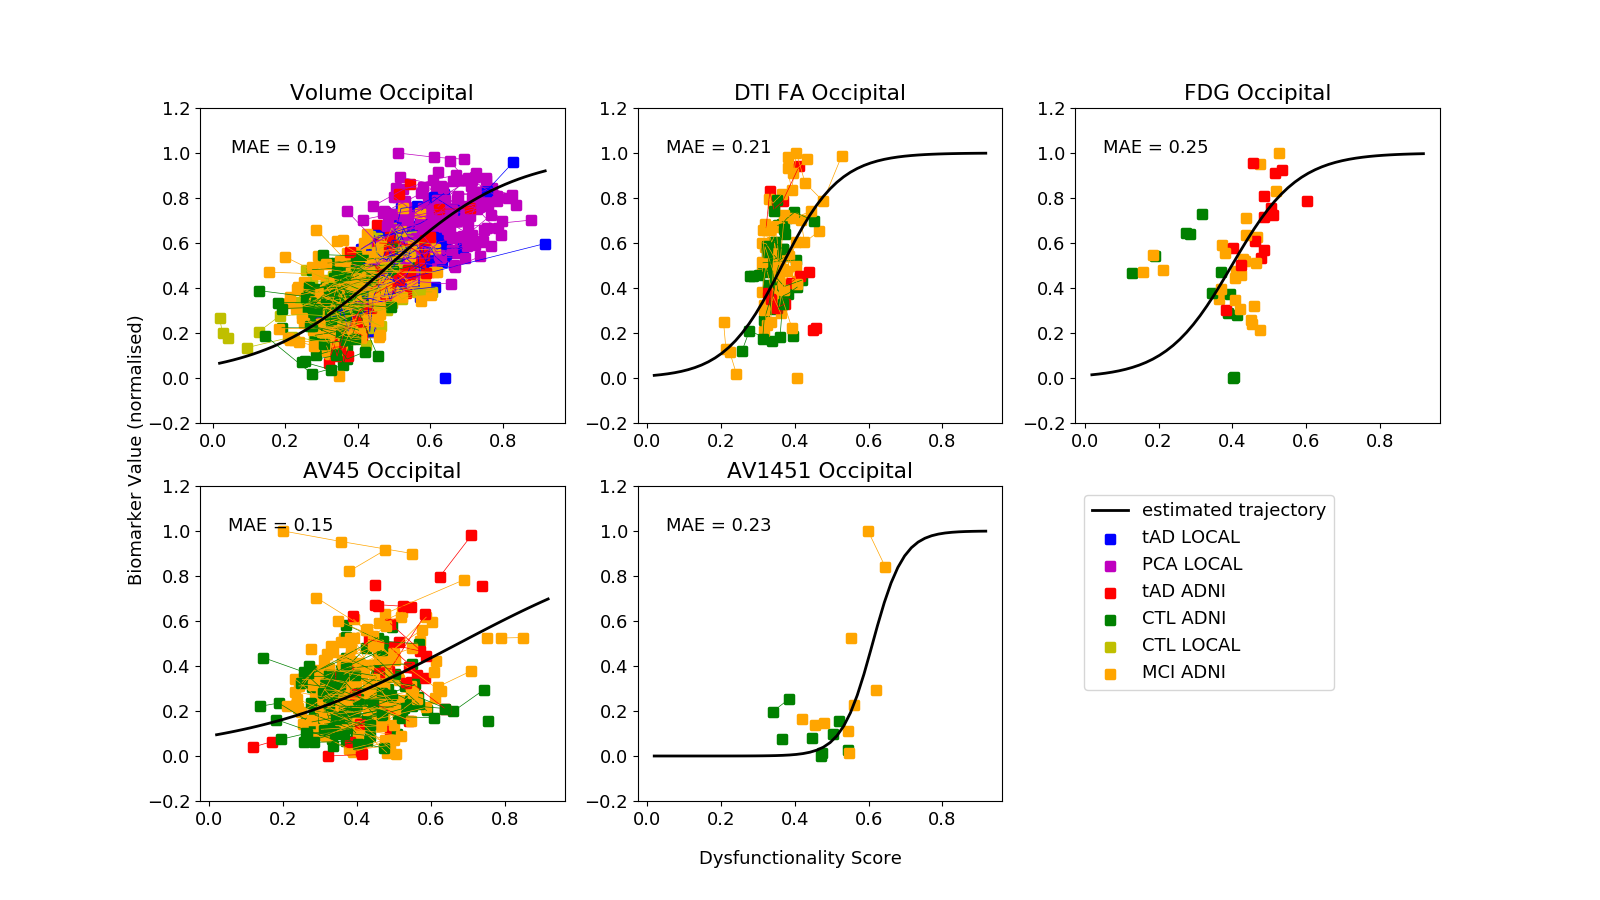
\includegraphics[width=0.8\textwidth, trim=90 0 110 0, clip]{\expFld/unit1_allTraj.png} 
% % \caption{}
% % \label{fig:occipUnit}
% \end{subfigure}
% 
% \begin{picture}(5,5)
% \put(0,20){\textbf{\Large{B}}}
% \end{picture}
% \begin{subfigure}{0.47\textwidth}
% \centering
% % typical AD\\
% 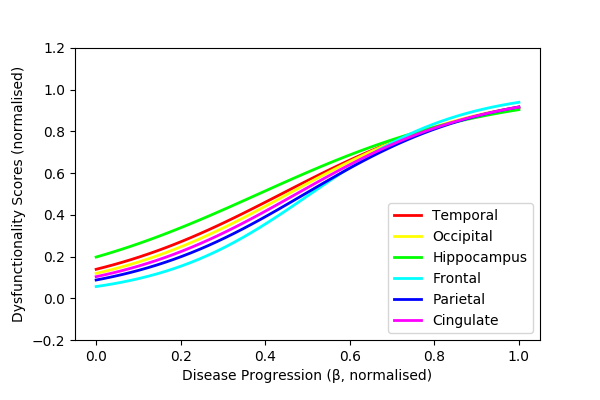
\includegraphics[width=0.8\textwidth, trim=0 0 0 20, clip]{\expFld/dis0_tAD_allTrajZeroOne.png} 
% % \caption{C}
% \end{subfigure}
% \begin{picture}(5,5)
% \put(0,20){\textbf{\Large{C}}}
% \end{picture}
% \begin{subfigure}{0.47\textwidth}
% \centering
% % PCA\\
% 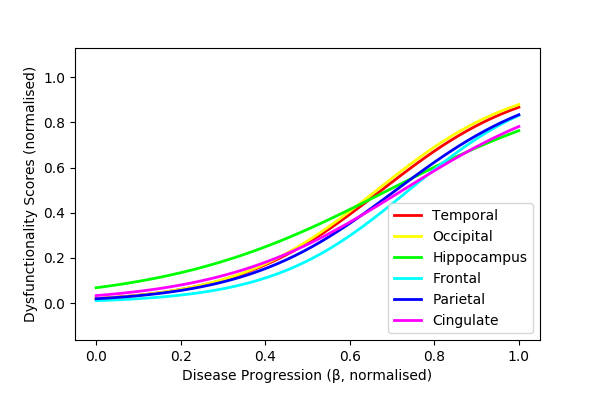
\includegraphics[width=0.8\textwidth, trim=0 0 0 20, clip]{\expFld/dis1_PCA_allTrajZeroOne.png}
% % \caption{PCA}
% \end{subfigure}
% \caption{(A) Estimated biomarker trajectories in the occipital agnostic unit, emulating the bottom-right subfigure from Fig \ref{fig:diagram}. Subject data from ADNI and DRC cohorts are also shown. The X-axis, defined as the occipital dysfunction score, represents the time-shifts (in months) of each subject. The Y-axis measures biomarker values (normalised). (B-C) Progression of dysfunction scores for (B) typical AD and (C) PCA, emulating top subfigures from Fig \ref{fig:diagram}.}
% \label{fig:pcaTadDisSpace}
% \end{figure}



% estimated (hypothetical) trajectories in PCA: DTI, FDG, AV45, AV1451.Volumetric trajectories were based on PCA MRI data.
\begin{figure}[htp]
 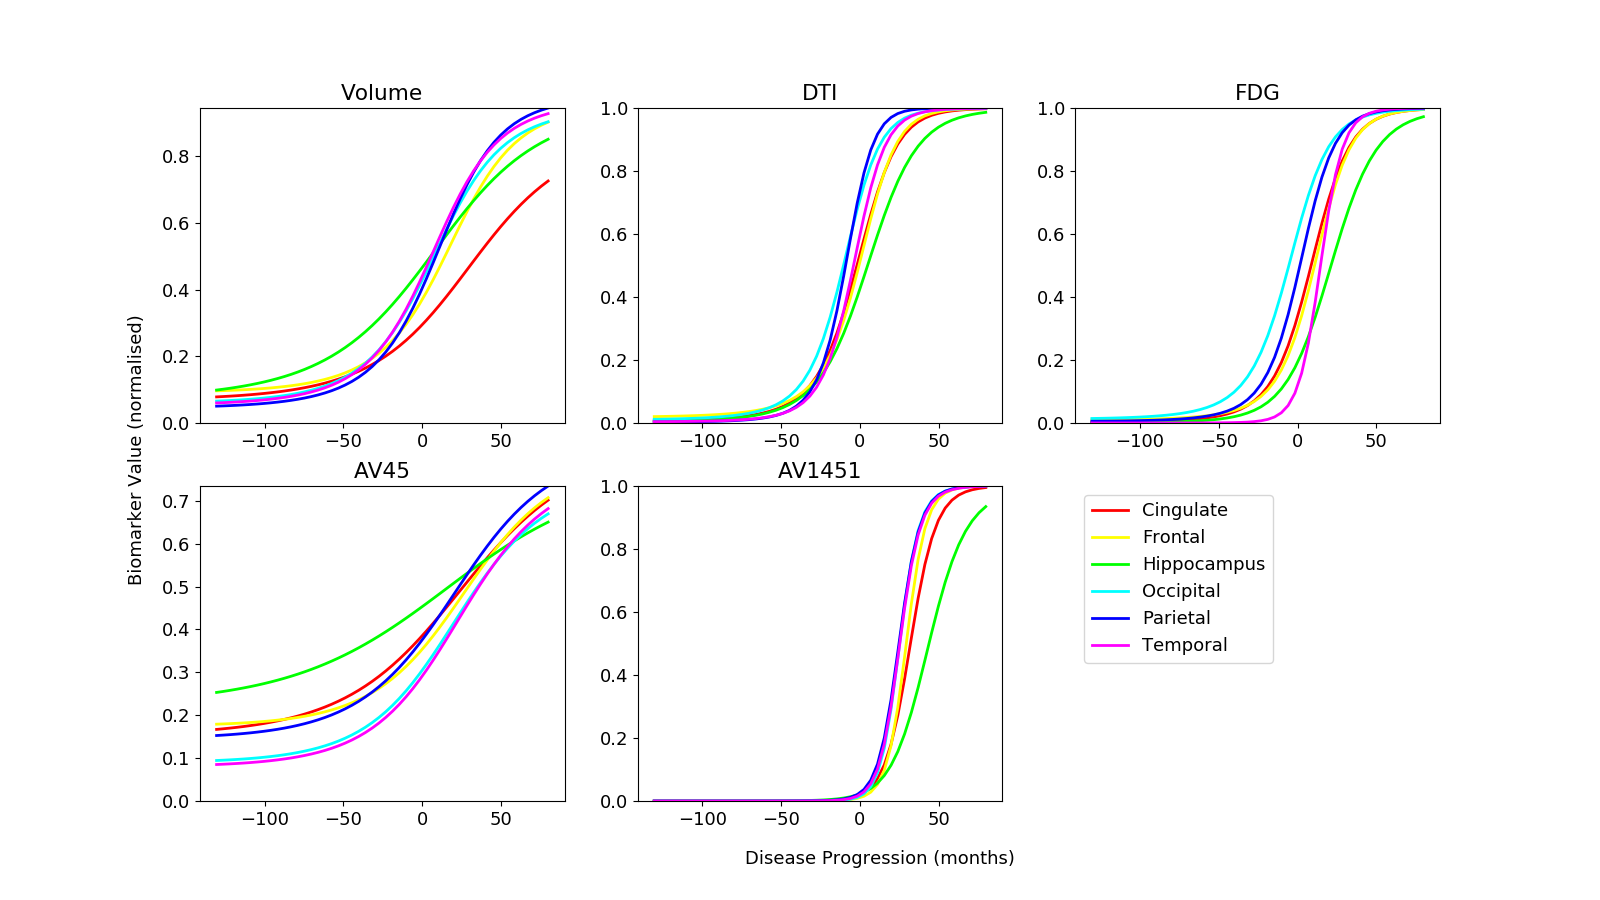
\includegraphics[width=\textwidth, trim=0 20 0 0, clip]{\expFld/trajDisSpaceOverlap_PCA_tad-drcTinyPen5_JMD.png}
 \caption{Estimated trajectories for the PCA cohort. The only data that were available were the MRI volumetric data. The dynamics of the other biomarkers has been inferred by the model using data from typical AD, and taking into account the different spatial distribution of pathology in PCA vs tAD.}
 \label{fig:PCAtrajByModality}
\end{figure}


\section{Validation on DTI Data in PCA}
\label{sec:dktResVal}

We validated our model using a separate test set of 20 DTI scans from controls and PCA patients from the DRC. We used DKT to predict the DTI biomarker values for the subjects within the unseen test set, using only their MRI biomarkers. Table \ref{sec:dktPerfMetrics} shows the prediction mean squared error (MSE) and rank correlation between the DKT-predicted biomarker values and the measured values. We computed the rank correlation in order to remove the effect of any systemic biases due to the completely different progressive disease and dataset that we are predicting on. We also show the same performance metrics for two simpler models: (1) a \emph{latent stage model}, as described in \cite{jedynak2012computational}, which assumes all tAD and PCA subjects follow the same progression and (2) a \emph{linear univariate model} that predicts the DTI biomarker based on the corresponding MRI biomarker, independently for each region.

The results from Table \ref{sec:dktPerfMetrics} indicate that the DKT prediction errors are relatively small for the frontal, occipital, temporal and parietal areas. Moreover, the rank correlations of the DKT predicted values are also high for the cingulate lobe and the hippocampus. In terms of model comparison, DKT has better performance than the linear model (all results significant with $p < 0.002$, Bonferroni corrected), since it uses information across all brain regions instead of assuming independence across regions. While DKT has similar performance to the latent stage model, it does not assume that the diseases have the same progression and it allows us to understand mechanisms that are shared between related diseases. 

\newcommand{\cw}{c}



\begin{table}
\centering
\fontsize{8}{10}\selectfont
\begin{tabular}{c | c c c c c c}
\textbf{Model} & \textbf{Cingulate} & \textbf{Frontal} & \textbf{Hippo.} & \textbf{Occip.} & \textbf{Parietal} & \textbf{Temporal}\\
& \multicolumn{6}{c}{\textbf{Prediction Error (MSE)}}\\
DKT & 0.09$\pm$0.04 & 0.03$\pm$0.01 & 0.18$\pm$0.03 & 0.04$\pm$0.02 & 0.06$\pm$0.02 & 0.04$\pm$0.02\\
Latent stage & 0.09$\pm$0.04 & 0.03$\pm$0.01 & 0.17$\pm$0.03 & 0.04$\pm$0.02 & 0.06$\pm$0.02 & 0.04$\pm$0.02\\
Linear & 0.05$\pm$0.02* & 0.15$\pm$0.04* & 0.09$\pm$0.03* & 0.07$\pm$0.03* & 0.07$\pm$0.02* & 0.07$\pm$0.02*\\
& \multicolumn{6}{c}{\textbf{Rank Correlation (Spearman rho)}}\\
DKT  & 0.76  & 0.48  & 0.76  & 0.55  & 0.55  & 0.33 \\
Latent stage & 0.76  & 0.49  & 0.80*  & 0.56  & 0.51*  & 0.33 \\
Linear & 0.48*  & 0.31*  & 0.64*  & 0.61*  & 0.57*  & 0.27* \\
\end{tabular}
% \normalfont
\caption[Performance evaluation of DKT and two simpler models]{Performance evaluation of DKT and two simpler models. (*) Statistically significant difference between the current model performance and DKT, based on a two-tailed t-test, Bonferroni corrected.}
% \end{footnotesize}
\label{sec:dktPerfMetrics}
\end{table}



\section{Discussion}
\label{sec:dktDis}

We presented DKT, a framework that enables, for the first time, joint modelling of biomarker progressions in multiple neurodegenerative diseases simultaneously. The framework allows the inference of biomarker trajectories in rare diseases, for which there is not enough data to allow estimation of such trajectories, and accounts for a different spatial distribution of pathology between distinct phenotypes. Our approach is also interpretable, enabling us to understand complex mechanisms underpinning these diseases.

% While we provided an example implementation of DKT using specific models of the biomarker trajectories, measurement noise and link function (the disease progression score), DKT should be considered as a general framework for joint modelling of biomarker trajectories within different diseases simultaneously. The actual implementation of DKT can thus be extended to use non-parametric trajectories, or more complex link functions that estimate not only subject time-shifts but also progression speed or higher order terms.
% 
% While here we have focused on Alzheimer's variants such as tAD and PCA, DKT can also be applied to other progressive neurodegenerative diseases of non-Alzheimer's type and even the normal ageing process. While we only used imaging data, cognitive tests can also be included in the disease-specific sub-models of DKT, or even allocated in the agnostic units of the regions that are responsible for those tasks.

Our work has several limitations: 1) DKT assumes all subjects within a disease follow the same trajectory, without considering heterogeneity within the disease population, 2) the allocation of biomarkers into agnostic units has to be done using \emph{a-priori} human knowledge, 3) DKT currently works only on extracted brain features, discarding important information present in the brain morphometry, 4) for validation, the synthetic experiment we ran was limited to only one setting of parameters mimicking the datasets from TADPOLE and the DRC centre and 5) the validation on patient data was also done only on a small set of 20 DTI scans, due to lack of multimodal data in PCA.

There are several potential avenues for further research: 1) to account for heterogeneity, DKT can be easily extended to include subject-specific effects; 2) improved schemes for biomarker allocation to agnostic units can take connectivity into account, or derive it from the data automatically; 3) to account for brain morphometry and connectivity, DKT can be extended into a fully spatio-temporal model, by estimating continuous changes in volumetric brain images -- in this case, each voxel can have an associated dysfunction score that is derived from measurements of various modalities from that voxel; 4-5) DKT can be further validated on more complex synthetic experiments with a range of parameter settings, as well as on patient data from ADNI, where the population could be \emph{a-priori} split into sub-groups with different progressions.

% As a key direction of further research, DKT can be used to understand novel mechanisms within a disease (e.g. AD variants), as well as across diseases (e.g. AD vs FTD). For AD variants in particular, one can study whether early biomarkers such as amyloid and tau have different dynamics compared to typical AD, and what these differences are. This can be done by choosing different a-priori allocations of biomarkers to agnostic units -- e.g. allocating amyloid and tau into one a shared agnostic unit, or otherwise directly to the disease specific models, thus making them dependent on the disease. The model with the best data fit or predictive power will indicate the most likely mechanism. 

%
% ---- Bibliography ---- 
% USE HARVARD STANDARD

\bibliographystyle{unsrtnat}
\begin{thebibliography}{5}

\bibitem{lorenzi2017disease}
Lorenzi, M., Filippone, M., Frisoni, G.B., Alexander, D.C., Ourselin, S. and Alzheimer's Disease Neuroimaging Initiative, 2017. Probabilistic disease progression modeling to characterize diagnostic uncertainty: application to staging and prediction in Alzheimer's disease. NeuroImage.


\bibitem{oxtoby2018}
Oxtoby, N.P., Young, A.L., Cash, D.M., Benzinger, T.L., Fagan, A.M., Morris, J.C., Bateman, R.J., Fox, N.C., Schott, J.M. and Alexander, D.C., 2018. Data-driven models of dominantly-inherited Alzheimer’s disease progression. Brain, 141(5), pp.1529-1544.

\bibitem{jedynak2012computational}
Jedynak, B.M., Lang, A., Liu, B., Katz, E., Zhang, Y., Wyman, B.T., Raunig, D., Jedynak, C.P., Caffo, B., Prince, J.L. and ADNI, 2012. A computational neurodegenerative disease progression score: method and results with the Alzheimer's disease Neuroimaging Initiative cohort. Neuroimage, 63(3), pp.1478-1486.

%\bibitem{iturria2016early}
%Iturria-Medina, Y., Sotero, R.C., Toussaint, P.J., Mateos-Pérez, J.M., Evans, A.C., Weiner, M.W., Aisen, P., Petersen, R., Jack, C.R., Jagust, W. and Trojanowki, J.Q., 2016. Early role of vascular dysregulation on late-onset Alzheimer's disease based on multifactorial data-driven analysis. Nature communications, 7, p.11934.


%\bibitem{young2014data}
%Young, A.L., Oxtoby, N.P., Daga, P., Cash, D.M., Fox, N.C., Ourselin, S., Schott, J.M. and Alexander, D.C., 2014. A data-driven model of biomarker changes in sporadic Alzheimer's disease. Brain, 137(9), pp.2564-2577.


\bibitem{young2018uncovering}
Young, A.L., Marinescu, R.V., Oxtoby, N.P., Bocchetta, M., Yong, K., Firth, N.C., Cash, D.M., Thomas, D.L., Dick, K.M., Cardoso, J. and van Swieten, J., 2018. Uncovering the heterogeneity and temporal complexity of neurodegenerative diseases with Subtype and Stage Inference. Nature communications, 9(1), p.4273.

%\bibitem{scelsi2018genetic}
%Scelsi, M.A., Khan, R.R., Lorenzi, M., Christopher, L., Greicius, M.D., Schott, J.M., Ourselin, S. and Altmann, A., 2018. Genetic study of multimodal imaging Alzheimer's disease progression score implicates novel loci. Brain.


\bibitem{hon2017towards}
Hon, M. and Khan, N., 2017. Towards Alzheimer's Disease Classification through Transfer Learning. arXiv preprint arXiv:1711.11117.


\bibitem{cheng2015domain}
Cheng, B., Liu, M., Zhang, D., Munsell, B.C. and Shen, D., 2015. Domain transfer learning for MCI conversion prediction. IEEE Transactions on Biomedical Engineering, 62(7), pp.1805-1817.

\bibitem{marinescu2018tadpole}
Marinescu, R.V., Oxtoby, N.P., Young, A.L., Bron, E.E., Toga, A.W., Weiner, M.W., Barkhof, F., Fox, N.C., Klein, S. and Alexander, D.C., 2018. TADPOLE Challenge: Prediction of Longitudinal Evolution in Alzheimer's Disease. arXiv:1805.03909.

\bibitem{jack2010hypothetical}
Jack Jr, C.R., Knopman, D.S., Jagust, W.J., Shaw, L.M., Aisen, P.S., Weiner, M.W., Petersen, R.C. and Trojanowski, J.Q., 2010. Hypothetical model of dynamic biomarkers of the Alzheimer's pathological cascade. The Lancet Neurology, 9(1), pp.119-128.

\bibitem{seeley2009neurodegenerative}
Seeley, W.W., Crawford, R.K., Zhou, J., Miller, B.L. and Greicius, M.D., 2009. Neurodegenerative diseases target large-scale human brain networks. Neuron, 62(1), pp.42-52.



%\bibitem{Ossenkoppele2014atrophy}
%Ossenkoppele, R., Cohn‐Sheehy, B.I., La Joie, R., Vogel, J.W., Möller, C., Lehmann, M., van Berckel, B.N., Seeley, W.W., Pijnenburg, Y.A., Gorno‐Tempini, M.L. and Kramer, J.H., 2015. Atrophy patterns in early clinical stages across distinct phenotypes of Alzheimer's disease. Human brain mapping, 36(11), pp.4421-4437.

\bibitem{crutch2012posterior}
Crutch, S.J., Lehmann, M., Schott, J.M., Rabinovici, G.D., Rossor, M.N. and Fox, N.C., 2012. Posterior cortical atrophy. The Lancet Neurology, 11(2), pp.170-178.


\end{thebibliography}

\clearpage

\end{document}

